% \section{Desenvolvimento espacial}

% Após o lançamento do \emph{Sputnik-1} \cite{nasa1957}, no final dos anos 50, e do início de uma série de satélites com na ordem de toneladas \cite{sputnik3}, a (\gls{urss}) demonstrou possuir foguetes com maior capacidade de carga que seus equivalentes no restante do globo.
% Tal feito foi fruto de um programa com alto nível de desenvolvimento, fundamentado em uma eficiente rede de pesquisa e inovação na área espacial. Esse avanço sugeria que o próximo passo natural seria a conquista da Lua e dos demais planetas do Sistema Solar \cite{betzler2024}.

% Porém, menos de uma década depois, os programas espaciais soviético e estadunidense estavam em níveis completamente diferentes.
% Enquanto o cosmonauta \emph{Komarov} havia morrido no primeiro teste de voo da \emph{Soyuz-1} \cite{zak2018}, a missão \emph{Apollo-8} realizava com sucesso a primeira circunavegação tripulada Terra-Lua \cite{nasaApollo8}.
% Em julho de 1969, o primeiro pouso lunar tripulado americano foi realizado \cite{nasaApollo11}; fato que consolidou o avanço tecnológico e estratégico dos Estados Unidos da América.
% Em contrapartida, as autoridades soviéticas anunciaram oficialmente que nunca houve um programa destinado ao pouso de cosmonautas na superfície lunar \cite{betzler2024}.

% Com o fim da URSS, em 1991, documentos secretos começaram a ser liberados, revelando informações que contradiziam as declarações oficiais.
% As razões para a falta de êxito da URSS em colocar cosmonautas na superfície lunar são variadas; abrangem desde limitações técnicas até questões políticas \cite{betzler2024}.
% A utilização dos foguetes como ferramenta estratégica ganhou impulso significativo na União Soviética após a Segunda Guerra Mundial, pois havia a percepção de que essa tecnologia poderia definir o equilíbrio de poder global. 
% Durante esse período, a pesquisa soviética esteve concentrada no desenvolvimento de tecnologias de foguetes voltadas para aplicações militares, como sistemas de decolagem assistida (JATO) \cite{glushko1973} e aeronaves movidas a motores-foguete.
% Projetos como o RP-318 \cite{RP318}, o BI-1 \cite{BI1} e o Malyutka \cite{Malyutka} foram exemplos iniciais desse esforço, mas o grande avanço veio com a captura e estudo das tecnologias alemãs após a guerra, especialmente os foguetes V-2.

% A partir deste momento, o trabalho relativo aos foguetes de grande alcance começou a tomar forma, com projetos como o \emph{Tikhonravov MK} e os mísseis D-1 e D-2 liderando o caminho.
% No entanto, as limitações de infraestrutura, recursos e conhecimento interno tornaram evidente a necessidade de uma abordagem mais organizada e estratégica. 
% Em resposta, a URSS iniciou em 1946 o desenvolvimento de mísseis de longo alcance \cite{siddiqi2004}, um decreto que estabelecia institutos de pesquisa especializados no desenvolvimento de foguetes, com a transferência de milhares de técnicos alemães para colaborar nesses esforços.
% Apesar dos avanços significativos, o programa espacial soviético enfrentava desafios estruturais, como a fragmentação de esforços entre diferentes projetistas e disputas internas por liderança.
% Contudo, o desenvolvimento dessas tecnologias ajudou a estabelecer a base para os marcos posteriores do programa espacial soviético, incluindo o lançamento do \emph{Sputnik-1} em 1957, que marcou o início da era espacial e consolidou a URSS como uma potência tecnológica global \cite{betzler2024}.

% A partir de 1956, o programa espacial soviético avançou, e o governo soviético definiu três metas principais \cite{betzler2024}: (I) lançar satélites artificiais com massa entre 1,80 e 2,50 toneladas até 1958, (II) desenvolver um satélite de reconhecimento não tripulado até 1970 e (III) realizar voos espaciais tripulados com duração de até uma semana até 1964.
% Esses objetivos serviam para consolidar a liderança soviética na exploração espacial, equilibrando as prioridades militares e científicas.
% A primeira meta, associada ao lançamento do satélite artificial terrestre (ISZ), foi iniciada com estudos em laboratório sobre o meio ambiente espacial.
% Em julho de 1956, o desenvolvimento do ISZ foi concluído, e a construção do satélite e seus sistemas de acompanhamento terrestre foi autorizada por um decreto em setembro do mesmo ano.
% No entanto, devido à pressão de lançar um satélite antes dos americanos, o projeto ISZ foi temporariamente adiado, e dois pequenos satélites, \emph{Sputnik-1} e \emph{Sputnik-2}, foram rapidamente construídos para cumprir essa meta \cite{betzler2024}.

% O lançamento do \emph{Sputnik-1} em 4 de outubro de 1957 \cite{nasaSputnik1} marcou o início da era espacial, tornando-se o primeiro satélite artificial a orbitar a Terra.
% Essa realização colocou a União Soviética à frente na corrida espacial, mas foi também uma demonstração de força militar e tecnológica em plena Guerra Fria.
% Pouco depois, o \emph{Sputnik-2} foi lançado, levando a bordo a cadela Laika \cite{nasaSputnik2}, o primeiro ser vivo a orbitar a Terra.

% \begin{figure}[H]
%     \label{fig_LABEL_AQUI}
% \centering
% 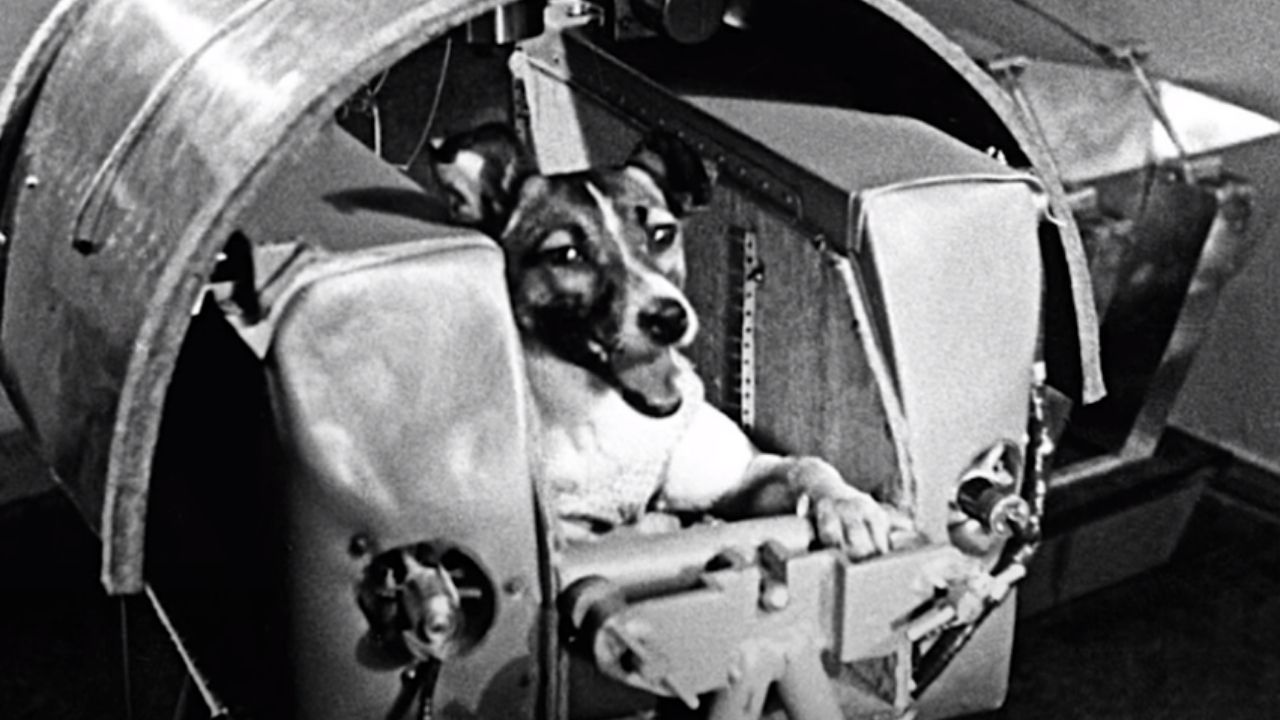
\includegraphics[width=1\linewidth]{1 Introducao/Imagens/Laika.jpg}
% \caption{Laika, o primeiro cachorro no espaço. Fonte: NASA.}
% \end{figure}

% Embora essas conquistas representassem avanços científicos, também eram fruto de disputas internas entre militares e civis sobre as prioridades do programa espacial.
% Enquanto os militares priorizavam satélites de reconhecimento, os civis advogavam pela importância de missões tripuladas \cite{betzler2024}.

% Em 1958, o projeto Vostok \cite{nasaVostok1} começou a ganhar forma, associado ao objetivo de realizar voos tripulados.
% Inicialmente, o trabalho ocorreu em paralelo ao projeto militar \emph{Zenit}, que visava o desenvolvimento de satélites de reconhecimento fotográfico.
% \emph{Korolev} defendeu que a tecnologia do Zenit \cite{astronautixZenit} poderia ser utilizada como base para os voos tripulados, o que resultou na unificação parcial dos esforços.
% O primeiro voo tripulado da \emph{Vostok} ocorreu em 12 de abril de 1961, com \emph{Yuri Gagarin}, tornando-se o primeiro ser humano a orbitar a Terra.
% A missão foi um marco na história da exploração espacial, quebrando recordes de velocidade e altitude para um veículo tripulado.
% No entanto, a missão enfrentou desafios, como falhas durante a reentrada, que exigiram que Gagarin ejetasse da cápsula antes do pouso.
% Apesar disso, a missão foi um sucesso e consolidou a posição soviética como líder na corrida espacial \cite{betzler2024}.

% O programa \emph{Vostok} foi seguido por novas iniciativas destinadas a expandir as capacidades soviéticas no espaço. As missões subsequentes buscavam reforçar o prestígio internacional da URSS.
% No entanto, os desafios estruturais do programa, como disputas entre projetistas, fragmentação de esforços e limitações de financiamento, começaram a impactar negativamente os avanços.
% Além disso, os EUA intensificaram seus esforços com o programa Apollo, superando a URSS na corrida para o pouso lunar.
% Apesar dessas dificuldades, o legado do programa espacial soviético permanece como uma das mais impressionantes realizações tecnológicas do século XX, destacando a capacidade de inovação em um contexto de recursos limitados e intensas pressões políticas \cite{betzler2024}.

% \subsection{Estação espacial Skylab (EUA)}

% A estação espacial \emph{Skylab} foi a primeira estação espacial americana e consolidou o avanço tecnológico do país após a corrida espacial contra a União Soviética.
% Desenvolvida a partir da terceira fase do programa \emph{Apollo}, a \emph{Skylab} foi projetada para utilizar os conhecimentos e tecnologias adquiridos durante as missões lunares, adaptando-os para objetivos científicos e de longo prazo em órbita terrestre.
% Lançada em 14 de maio de 1973, a \emph{Skylab} tinha como missão principal realizar experimentos científicos em microgravidade, estudar a Terra e o Sol, além de compreender os efeitos do ambiente espacial em seres humanos durante estadias prolongadas \cite{nasaSkylab}.

% \begin{figure}[H]
%     \centering
%     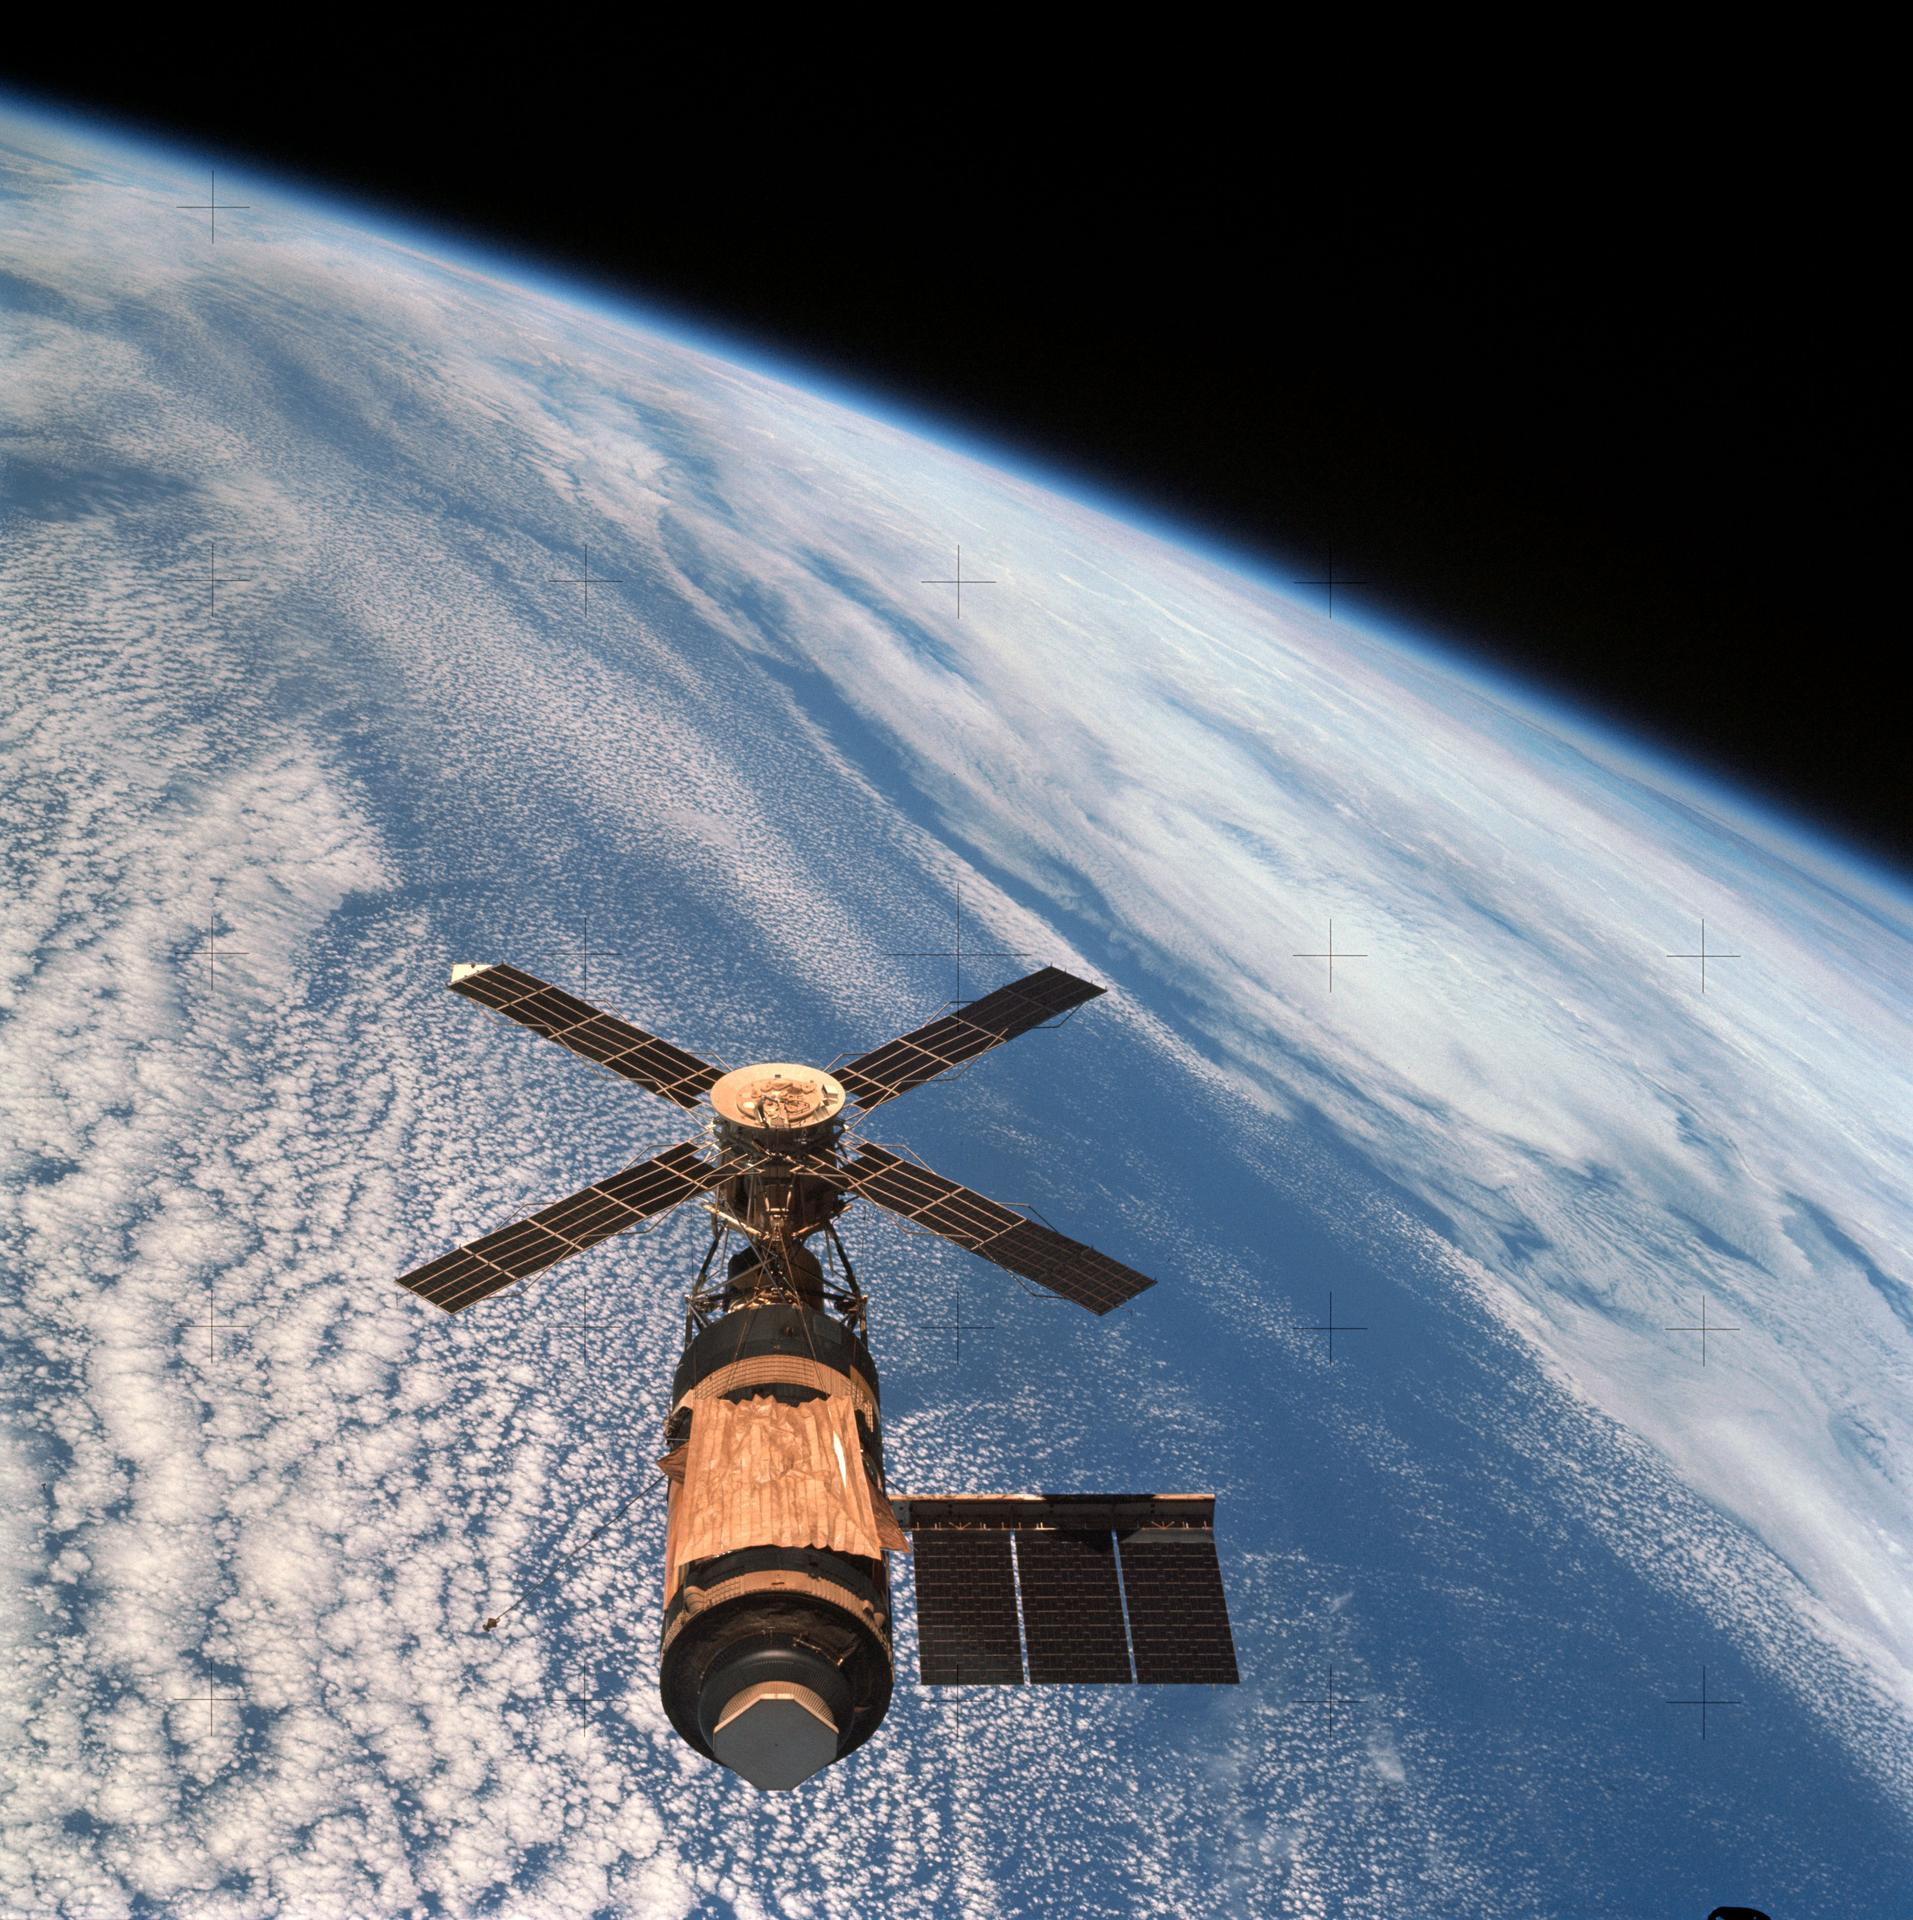
\includegraphics[width=0.75\linewidth]{1 Introducao/Imagens/Skylab NASA.jpg}
%     \caption{Estação Espacial Skylab. Fonte: NASA.}
%     \label{fig_SkylabFoto}
% \end{figure}

% A estrutura da \emph{Skylab} era baseada no segundo estágio de um foguete \emph{Saturn V} modificado, transformado em um laboratório espacial.
% Isso permitiu reduzir custos e aproveitar a infraestrutura existente.
% A estação espacial era dividido em módulos, incluindo o laboratório orbital, o módulo de múltiplos usos, a estação de controle e o módulo solar, além disso, a estação contava com painéis solares que forneciam energia para os experimentos e para a manutenção do ambiente interno.
% Os avanços tecnológicos implementados permitiram que a tripulação realizasse experimentos complexos, observações solares com o uso de telescópios especializados, estudos de ciências da vida e experimentos em física de fluidos \cite{nasaSkylab}.

% As missões tripuladas para a \emph{Skylab} foram realizadas por meio de espaçonaves \emph{Apollo} modificadas que transportaram astronautas para estadias de longa duração na estação.
% Três tripulações visitaram a \emph{Skylab} entre 1973 e 1974, cada uma estabelecendo recordes crescentes de permanência em órbita \cite{nasaSkylab}.

% Apesar de seu sucesso científico, a \emph{Skylab} enfrentou desafios operacionais desde o início.
% Durante o lançamento, a estação sofreu danos, incluindo a perda de um escudo térmico e um dos seus principais painéis solares \cite{nasaSkylab2}.
% Esses problemas comprometeram a capacidade da estação de gerar energia e regular sua temperatura interna.
% No entanto, com o apoio de engenheiros em terra e a habilidade da primeira tripulação, reparos improvisados foram realizados: fizeram a instalação de um escudo solar para reduzir a temperatura interna e a liberação manual de um painel solar preso \cite{nasaSkylab}.

% Embora a estação espacial \emph{Skylab} tenha superado muitos dos seus desafios iniciais, a estação não estava preparada para resistir indefinidamente em órbita.
% Em 1979, após anos de abandono devido à falta de capacidade da NASA para realizar missões de manutenção com o Space Shuttle, a \emph{Skylab} reentrou na atmosfera terrestre, com partes de seus destroços caindo na Austrália Ocidental \cite{nasaSkylabReentry}.
% O legado da \emph{Skylab} permanece significativo, pois serviu como uma plataforma de aprendizado para o desenvolvimento de estações espaciais maiores e mais modernas, além de estabelecer os alicerces para programas como o da ISS. 
% Além disso, as descobertas científicas realizadas no Skylab continuam a influenciar a compreensão de questões fundamentais sobre a vida e o trabalho no espaço \cite{nasaSkylab}.

% \subsection{Colaboração internacional}

% A Estação Espacial Internacional (ISS) é uma das maiores realizações da cooperação internacional na exploração espacial. Desde sua montagem em 1998, a ISS tem servido como um laboratório de microgravidade e um centro de pesquisa científica em órbita terrestre. Ela foi desenvolvida em parceria entre cinco agências espaciais: NASA (Estados Unidos), Roscosmos (Rússia), ESA (Europa), JAXA (Japão) e CSA (Canadá), representando um marco na colaboração tecnológica global. A ISS orbita a Terra a uma altitude média de 400 quilômetros e completa aproximadamente 16 órbitas por dia, oferecendo uma plataforma única para experimentos científicos que não seriam possíveis na Terra \cite{nasaISS}.

% \begin{figure}[H]
%     \centering
%     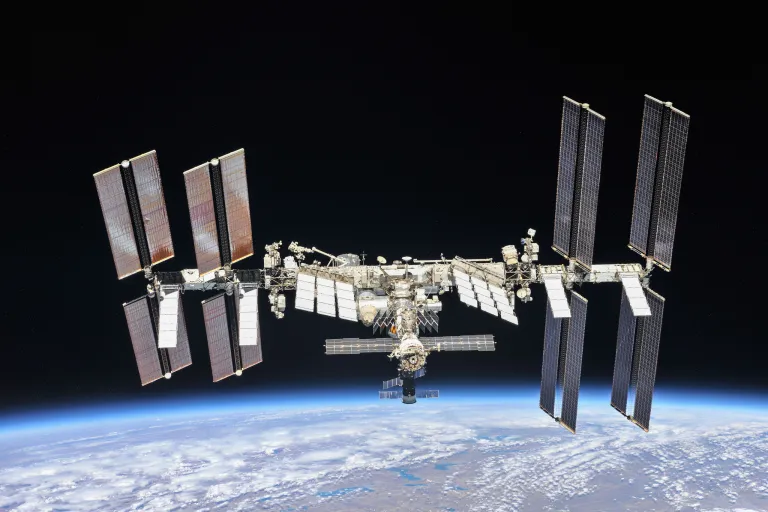
\includegraphics[width=0.75\linewidth]{1 Introducao/Imagens/ISS NASA.png}
%     \caption{A Estação Espacial Internacional (ISS) orbitando a Terra. Fonte: NASA.}
%     \label{fig_ISSfoto}
% \end{figure}

% A principal contribuição da ISS é no avanço da ciência em diversas áreas, incluindo biologia, física, ciência dos materiais e astronomia. Pesquisas realizadas a bordo da estação têm proporcionado visões valiosas sobre os efeitos de longo prazo da microgravidade no corpo humano, contribuindo diretamente para o planejamento de missões de exploração a longo prazo, como para Marte. Além disso, a ISS tem desempenhado um papel importante no teste de tecnologias necessárias para operações espaciais prolongadas, incluindo sistemas de suporte à vida, reciclagem de água e geração de energia solar \cite{nasaISS}.

% A construção da ISS foi um empreendimento monumental, exigindo mais de 30 missões de montagem realizadas por naves espaciais como o Space Shuttle. A estação é composta por diversos módulos conectados, cada um projetado para funções específicas, como laboratórios de pesquisa, áreas de habitação e módulos de suporte técnico. O sistema de acoplamento da ISS é outro elemento importante, permitindo a chegada de veículos de carga e tripulação, como as cápsulas Dragon \cite{spacexDragon}, Cygnus \cite{northropCygnus} e Soyuz \cite{nasaSoyuz}. Essas capacidades garantem o fornecimento contínuo de suprimentos e a troca de tripulações, que geralmente permanecem em períodos de seis meses \cite{nasaISS}.

% Além de suas contribuições científicas, a ISS também promove a diplomacia e a cooperação internacional. Cientistas e astronautas de diversas nações trabalham juntos para realizar pesquisas e operações diárias, criando um ambiente de colaboração global. A estação também serve como uma ferramenta educacional, inspirando novas gerações de cientistas e engenheiros por meio de programas de divulgação e parcerias com instituições educacionais \cite{nasaISS}.

% À medida que a ISS se aproxima do fim de sua operação planejada, prevista para 2030 \cite{nasaISSPlan}, as agências espaciais globais estão avaliando o futuro da exploração em órbita terrestre. A estação estabeleceu as bases para futuras estações espaciais comerciais e para missões ainda mais ambiciosas no espaço profundo. O legado da ISS, portanto, vai além das suas contribuições científicas e tecnológicas, representando o potencial da humanidade de trabalhar em conjunto para objetivos comuns \cite{nasaISS}.

%%%%%%%%%%%%%%%%%%%%%%%%%%%%%%%%%%%%%%%%%%%%%%%%%%%%%%%%%%%%%%%

\section{Desenvolvimento espacial}

O desenvolvimento espacial do período pós-guerra permitiu evoluir tecnologias espaciais, como a inserção orbital e operações orbitais contínuas, nas quais \gls{rvdb} se torna capacidade habilitadora.
O lançamento do \emph{Sputnik-1} \cite{nasaSputnik1} e a sequência de satélites maiores \cite{sputnik3} comprovaram a evolução das missões de lançamento e da infraestrutura tecnológica.
Programas estes que foram impulsionadas por programas nacionais apoiados em redes de pesquisa e inovação.
% Neste contexto, as iniciativas espaciais com aplicações estratégicas e militares também contribuíram para a evolução de sistemas de foguetes e para a expansão das metas espaciais \cite{glushko1973,siddiqi2004,betzler2024}.
Neste contexto, as iniciativas espaciais com aplicações estratégicas e militares também contribuíram para a evolução de sistemas de foguetes e para a expansão das metas espaciais \cite{betzler2024}.

A partir do início da década de 1960, a exploração espacial tripulada e a construção de plataformas orbitais passaram a exigir, além do acesso ao espaço, a capacidade de conduzir operações de proximidade, como o encontro orbital, aproximação controlada e acoplamento.
Ainda que o avanço tecnológico no setor espacial tenha ocorrido em ritmos distintos entre URSS e EUA \cite{betzler2024}, a experiência acumulada em missões tripuladas exteriorizou os riscos e a necessidade de robustez operacional em sistemas críticos (por exemplo, em programas iniciais como \emph{Soyuz-1} \cite{zak2018}), enquanto marcos como \emph{Apollo-8} e \emph{Apollo-11} consolidaram a transição para arquiteturas de missão mais complexas \cite{nasaApollo8,nasaApollo11}.
% Paralelamente, o programa soviético avançou na capacidade de voo tripulado e no aproveitamento de plataformas derivadas de projetos de reconhecimento, como no desenvolvimento associado a \emph{Vostok} e \emph{Zenit} \cite{nasaVostok1,astronautixZenit,betzler2024}.
Paralelamente, o programa soviético avançou na capacidade de voo tripulado e no aproveitamento de plataformas derivadas de projetos de reconhecimento, como no desenvolvimento associado a \emph{Vostok} e \emph{Zenit} \cite{nasaVostok1,astronautixZenit}.
Assim, a relevância obtida com a evolução tecnológica desse período estabeleceu as condições para operações orbitais recorrentes e contínuas, nas quais, o \gls{rvdb} se torna importante para que ocorra
(i) o acesso a estações espaciais,
(ii) logística de tripulação e suprimentos e
(iii) manutenção e/ou expansão de infraestrutura em órbita \cite{betzler2024}.